% Locomotion-policy background + related-work figure.
% Standalone-compiles on its own; \input{} the tikzpicture body into the
% paper/thesis main.tex once finalized.
%
% Structure (3 tiers, top to bottom):
%   1. Generic locomotion RL loop (shared vocabulary).
%   2. Zoom on the action-generation step: the two families of intervention
%      prior work applies there (structured exploration vs. frozen prior+residual).
%   3. Branch on prior *source* for family 2 -- this is the punchline: every
%      existing source is circular (built from an existing controller),
%      EMG is the only one that isn't.
%
% To trim for the ICLR paper (space-constrained): comment the DEP-RL /
% Lattice / reward-shaping annotations in tier 2 and keep just the
% LAP / Park et al. / SAR / EMG branch in tier 3.
\documentclass[tikz,border=4pt]{standalone}
\usepackage{amsmath}
\usepackage{tikz}
\usetikzlibrary{shapes.geometric,arrows.meta,positioning,fit,backgrounds,decorations.pathreplacing,calc}

\begin{document}
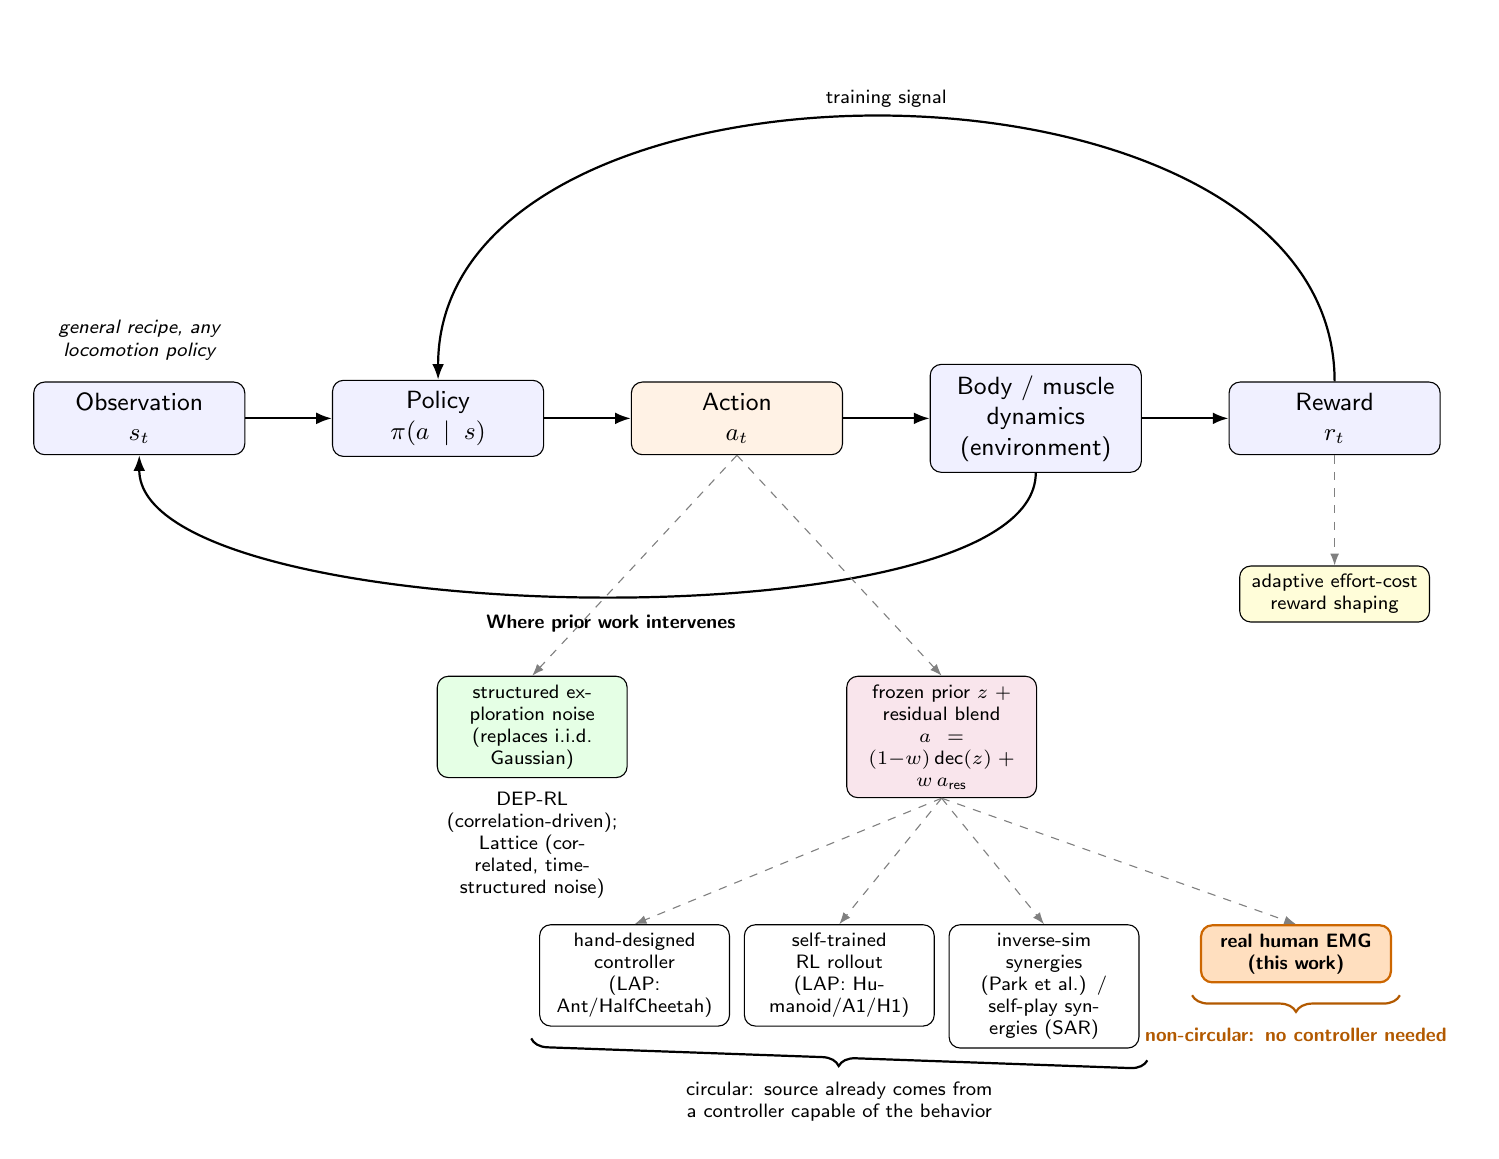
\begin{tikzpicture}[
  font=\sffamily\small,
  box/.style={draw, rounded corners, fill=blue!6, minimum height=0.9cm,
              text width=2.4cm, align=center, inner sep=4pt},
  smallbox/.style={draw, rounded corners, minimum height=0.7cm,
              text width=2.2cm, align=center, inner sep=3pt, font=\sffamily\scriptsize},
  circ/.style={draw, circle, fill=orange!15, minimum size=0.9cm, align=center, font=\scriptsize},
  arr/.style={-{Latex[length=2mm]}, thick},
  annot/.style={font=\sffamily\scriptsize, align=center, text width=2.6cm},
  leader/.style={-{Latex[length=1.5mm]}, dashed, gray},
]

%% ---------- TIER 1: generic loop ----------
\node[box] (obs) at (0,0) {Observation\\ $s_t$};
\node[box, right=1.1cm of obs] (pol) {Policy\\ $\pi(a\mid s)$};
\node[box, right=1.1cm of pol, fill=orange!10] (act) {Action\\ $a_t$};
\node[box, right=1.1cm of act] (env) {Body / muscle dynamics\\ (environment)};
\node[box, right=1.1cm of env] (rew) {Reward\\ $r_t$};

\draw[arr] (obs) -- (pol);
\draw[arr] (pol) -- (act);
\draw[arr] (act) -- (env);
\draw[arr] (env) -- (rew);
\draw[arr] (rew.north) to[out=90,in=90] node[above,font=\sffamily\scriptsize]{training signal} (pol.north);
\draw[arr] (env.south) to[out=-90,in=-90,looseness=0.5] (obs.south);

\node[annot, above=0.15cm of obs] {\itshape general recipe, any locomotion policy};

%% ---------- TIER 2: zoom on action generation ----------
\node[annot, below=1.9cm of act, xshift=-1.6cm, text width=4.5cm] (t2title)
  {\bfseries Where prior work intervenes};

\node[smallbox, fill=green!10, below=2.8cm of act, xshift=-2.6cm] (explore)
  {structured exploration noise\\ (replaces i.i.d.\ Gaussian)};
\node[smallbox, fill=purple!10, below=2.8cm of act, xshift=2.6cm] (frozen)
  {frozen prior $z$ + residual blend\\ $a=(1{-}w)\,\text{dec}(z)+w\,a_{\text{res}}$};

\draw[leader] (act.south) -- (explore.north);
\draw[leader] (act.south) -- (frozen.north);

\node[annot, below=0.05cm of explore, text width=2.4cm] {DEP-RL (correlation-driven);\\ Lattice (correlated, time-structured noise)};

%% ---------- TIER 3: branch on prior *source* ----------
\node[smallbox, below=1.6cm of frozen, xshift=-3.9cm] (src1)
  {hand-designed controller\\ (LAP: Ant/HalfCheetah)};
\node[smallbox, below=1.6cm of frozen, xshift=-1.3cm] (src2)
  {self-trained RL rollout\\ (LAP: Humanoid/A1/H1)};
\node[smallbox, below=1.6cm of frozen, xshift=1.3cm] (src3)
  {inverse-sim synergies\\ (Park et al.) /\\ self-play synergies (SAR)};
\node[smallbox, below=1.6cm of frozen, xshift=4.5cm, fill=orange!25, draw=orange!80!black, thick] (src4)
  {\bfseries real human EMG\\ (this work)};

\foreach \s in {src1,src2,src3,src4}
  \draw[leader] (frozen.south) -- (\s.north);

% circularity bracket under the first three
\draw[decorate, decoration={brace, amplitude=6pt, mirror}, thick]
  ($(src1.south west)+(-0.1,-0.15)$) -- ($(src3.south east)+(0.1,-0.15)$)
  node[midway, below=8pt, annot, text width=6cm]
  {circular: source already comes from a controller capable of the behavior};

\draw[decorate, decoration={brace, amplitude=6pt, mirror}, thick, orange!70!black]
  ($(src4.south west)+(-0.1,-0.15)$) -- ($(src4.south east)+(0.1,-0.15)$)
  node[midway, below=8pt, annot, text width=4.2cm, font=\sffamily\scriptsize\bfseries]
  {non-circular: no controller needed};

%% ---------- reward-shaping annotation (tier 2, optional for thesis) ----------
\node[smallbox, fill=yellow!15, below=1.4cm of rew] (rewshape)
  {adaptive effort-cost\\ reward shaping};
\draw[leader] (rew.south) -- (rewshape.north);

\end{tikzpicture}
\end{document}
